\section{Algoritmos y aplicaciones}
\label{sec:algoritmos}

Dado el problema planteado, su solución implica el uso de algoritmos de visión
por computadora que permitan automatizar la identificación de flores, como en
las aplicaciones descritas en la sección de contexto. A continuación se explica
por qué los algoritmos clásicos no son adecuados y qué arquitecturas proponemos.

\subsection{Algoritmos clásicos de aprendizaje automático}

Algoritmos como $k$ vecinos más cercanos (KNN), \textit{Random Forest} (RF) y
máquinas de soporte vectorial (SVM) funcionan de manera correcta con datos
tabulares, pero se adaptan mal a imágenes. Una imagen de $224\times224$ píxeles
RGB tiene $224\cdot224\cdot3 = 150{,}528$ valores, y una de $112\times112$, la
resolución que usamos, tiene 37,632. Tratar cada valor como una característica
independiente genera varios problemas:

\begin{itemize}
\item \textbf{KNN.} En espacios con tantas dimensiones, las distancias entre
puntos dejan de ser informativas (la llamada maldición de la dimensionalidad).
Además, la distancia entre píxeles no refleja similitud visual: dos fotos de la
misma flor con un ligero desplazamiento o distinta iluminación quedan muy lejos
entre sí. KNN guarda todo el conjunto de entrenamiento y calcula distancias
contra todas las imágenes en cada predicción, lo cual es costoso.
\item \textbf{Random Forest.} Cada árbol divide los datos según el valor de un
solo píxel, sin considerar su posición relativa ni sus vecinos, por lo que no
puede capturar formas ni texturas.
\item \textbf{SVM.} Con kernel, el costo de entrenamiento crece rápidamente con
el número de imágenes y de dimensiones, y sobre píxeles crudos no es invariante
a desplazamientos, rotaciones ni cambios de escala, que en este conjunto son
comunes.
\end{itemize}

Estos métodos requerirían extraer características manualmente (bordes, color,
textura) antes de clasificar. Las redes convolucionales evitan este paso, ya que
aprenden las características directamente de los píxeles.

\begin{figure}[htbp]
    \centering
    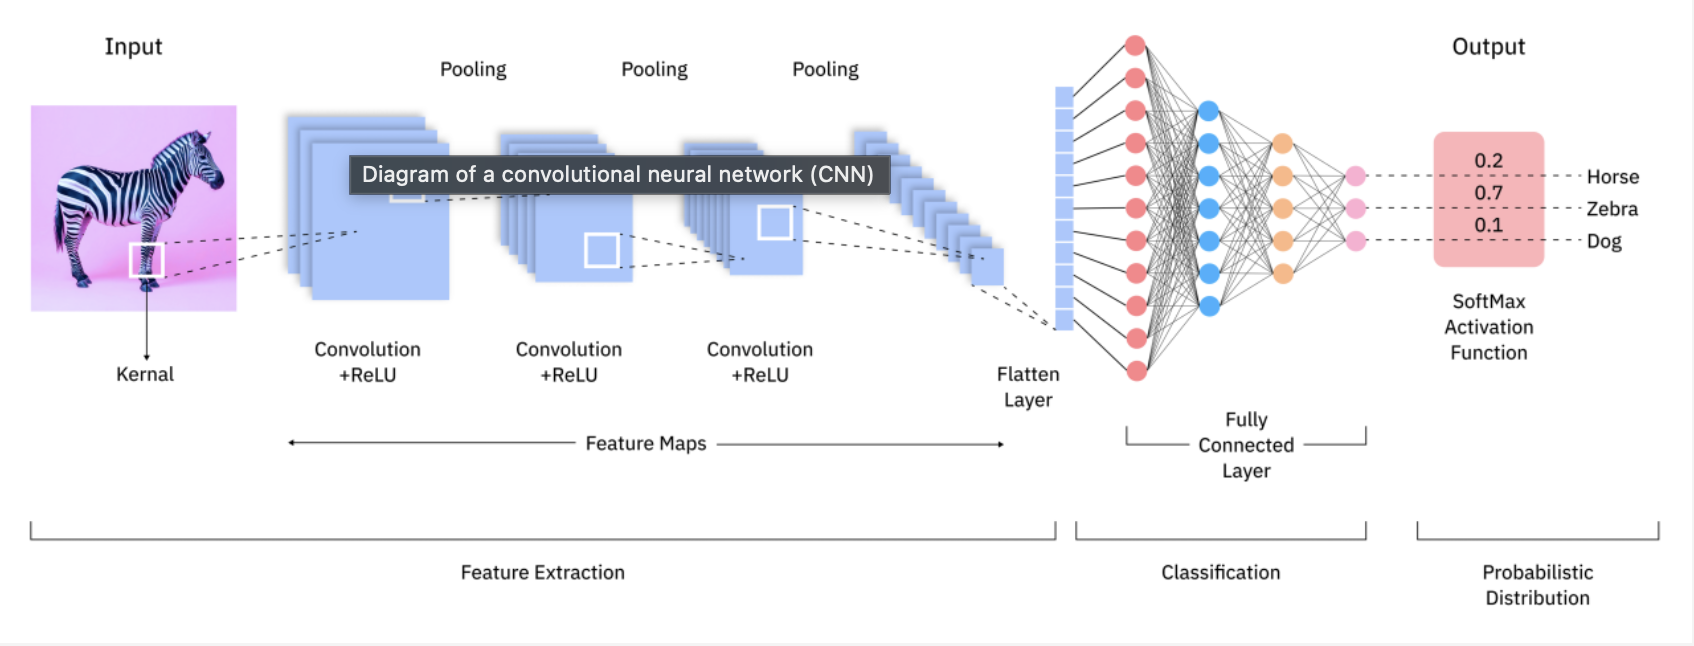
\includegraphics[width=\columnwidth]{cnn_diagram.png}
    \caption{Esquema de una red convolucional: las convoluciones extraen
    características de la imagen y las capas densas las usan para clasificar
    \autocite{ibmWhatImage}.}
    \label{fig:cnn_diagram}
\end{figure}

\subsection{CNN propia entrenada desde cero}
\label{sec:cnn-propia}

Las redes neuronales convolucionales (CNN) son una alternativa especialmente
adecuada para este problema debido a su capacidad para procesar información
espacial (Figura~\ref{fig:cnn_diagram}). Mediante filtros convolucionales pueden
aprender automáticamente características de las imágenes, como bordes, texturas
y formas. En las capas internas pueden emplearse funciones de activación como
ReLU, mientras que Softmax puede utilizarse en la salida para representar las
probabilidades de las distintas clases.

Nuestra primera propuesta es una CNN propia con cuatro bloques convolucionales
(de 32 a 256 filtros), \textit{Global Average Pooling}, una capa densa de 256
neuronas con \textit{dropout} de 0.5 y una capa de salida \textit{softmax} de
104 neuronas. Tiene 480,936 parámetros entrenables
(Tabla~\ref{tab:parametros}) y recibe imágenes de $112\times112$ píxeles.

Elegimos empezar desde cero por tres razones. Es ligera: se entrena en unos 20
minutos en una GPU de una Mac M4, lo que permite repetir experimentos. Permite
estudiar de forma controlada el efecto de la regularización, de la profundidad
y del desbalance, porque todo lo que la red sabe lo aprende de estos datos. Y
sirve como línea base para medir cuánto aportaría un modelo preentrenado. Su
reto es que, con un promedio de solo 123 imágenes por clase, existe riesgo de
sobreajuste, tema que se mide en la Sección~\ref{sec:res-regularizacion}.

\subsection{Transferencia de aprendizaje}
\label{sec:transfer}

La segunda alternativa es partir de una red ya entrenada en ImageNet
\autocite{deng2009imagenet}, con 1.2 millones de imágenes de 1,000 categorías, y
ajustarla a las flores. Dos arquitecturas concretas son adecuadas:

\begin{itemize}
\item \textbf{ResNet50} \autocite{he2016resnet}: 50 capas con conexiones
residuales, que suman la entrada de cada bloque a su salida. Esto permite
entrenar redes muy profundas sin que el gradiente se desvanezca. Tiene unos 25
millones de parámetros y usa entradas de $224\times224$.
\item \textbf{EfficientNetB0} \autocite{tan2019efficientnet}: escala de forma
equilibrada la profundidad, el ancho y la resolución de la red. Con unos 5.3
millones de parámetros y entradas de $224\times224$ logra una exactitud en
ImageNet comparable a la de ResNet50 con cinco veces menos parámetros.
\end{itemize}

Estas redes sirven con unas 123 imágenes por clase porque no aprenden desde
cero: sus primeras capas ya detectan bordes, texturas y formas generales, y
solo hace falta ajustar las últimas capas (o reemplazar la de salida) para
distinguir las 104 clases. Así, la poca información por clase se usa para
aprender lo específico de cada flor y no lo general de una imagen. Además, su
entrada de $224\times224$ coincide con una de las resoluciones del conjunto y
conserva detalles que se pierden a $112\times112$.

Conviene probar la transferencia de aprendizaje cuando la CNN propia deja de
mejorar con más regularización o capacidad, que es lo que muestran los
resultados de este trabajo (Sección~\ref{sec:analisis}). El repositorio ya
incluye la configuración para EfficientNetB0, pero su corrida no se completó
por tiempo de cómputo, por lo que queda como trabajo futuro.

\subsection{Aplicaciones y alcance}

Un modelo como el de este trabajo podría integrarse en una aplicación que, a
partir de una fotografía, sugiera la flor más probable y sus alternativas, al
estilo de iNaturalist \autocite{inaturalist}, o en herramientas educativas para
jardines botánicos y escuelas. En ambos casos funcionaría como apoyo a una
persona y no como identificación definitiva.

Cabe aclarar que el modelo solo puede reconocer las 104 clases presentes en el
conjunto de datos: ante una flor de otra especie, elegirá la más parecida de
esas 104. Una aplicación real más amplia requeriría entrenarlo con una variedad
mucho mayor de especies y detectar cuándo una imagen no pertenece a ninguna
clase conocida.
